\chapter{Optimizing patients travel}

\section{Context}

% Early diagnosis importance
Between 30 and 50\% of cancers can currently be prevented by avoiding risk factors and implementing prevention strategies. Many cancers have a high chance of cure if diagnosed early and treated appropriately.

% Impact of travel on earth
Treatment and travel \cite{weiss_global_2020,brundisini_chronic_2013,kelly_are_2016,salerno_understanding_2022}.
Impact of traveling on cancer patients \cite{payne_impact_2000,flytkjaer_virgilsen_cancer_2019,virgilsen_travel_2019,payne_impact_2000,ambroggi_distance_2015}.
Air pollution due to car emissions increases the risk of developing lung cancer \cite{raaschou-nielsen_air_2013}.

% Transportation and GHG
The transport sector is the number one emitter of greenhouse gases in France, with 30\% of emissions. The value attributed to the emissions generated are split between the operating phase (fuel combustion) and the upstream phase (fuel extraction, refining and distribution). The number one greenhouse gas emitted by the transport industry is carbon dioxide \ac{co2}.
France has set itself the objective of reducing its emissions by 75\% by the year 2050. In this scenario, patients travel will be impacted.

% Health and climate change
The \ac{ipcc}, warned that global warming will significantly affect hundreds of millions of people \cite{change_climate_2015}.
The Lancet Countdown on health and climate change started to review annually the relation between health and climate change \cite{watts_2020_2021}.
The health care sector is an important contributor to \ac{co2} emissions. International comparison of health care carbon footprints: on average, the health carbon footprint in 2014 constituted 5.5\% of the total national carbon footprint equivalent to the food industry in some countries \cite{pichler_international_2019}.
A large share of these carbon emissions is due to patients journeys \cite{andrews_carbon_2013,nicolet_what_2022} because most patients travel by car \cite{forner_carbon_2021}. With regionalization of care, patients are incentivized to be treat-ed in large hospitals for better outcome \cite{eskander_health_2016}. Such hospitals are in urban areas, and the populations living in rural areas will have to travel longer to reach these centers, resulting in higher carbon emissions.

% Routing optimization
Optimization of patients' routes would have multiple benefits: reduce the travel burden for patients; lower the carbon footprint.
Hospital recommender system \cite{zhang_idoctor_2017,han_hybrid_2018,narducci_recommender_2015,hoens_reliable_2010,tran_recommender_2021}.

% Towards a more transparent healthcare
Greater information seeking among cancer survivors \cite{finney_rutten_cancer-related_2016}. Providing tools for patients to understand where they are treated and which hospital they should go to.

\section{Results}

\begin{figure}[h]
    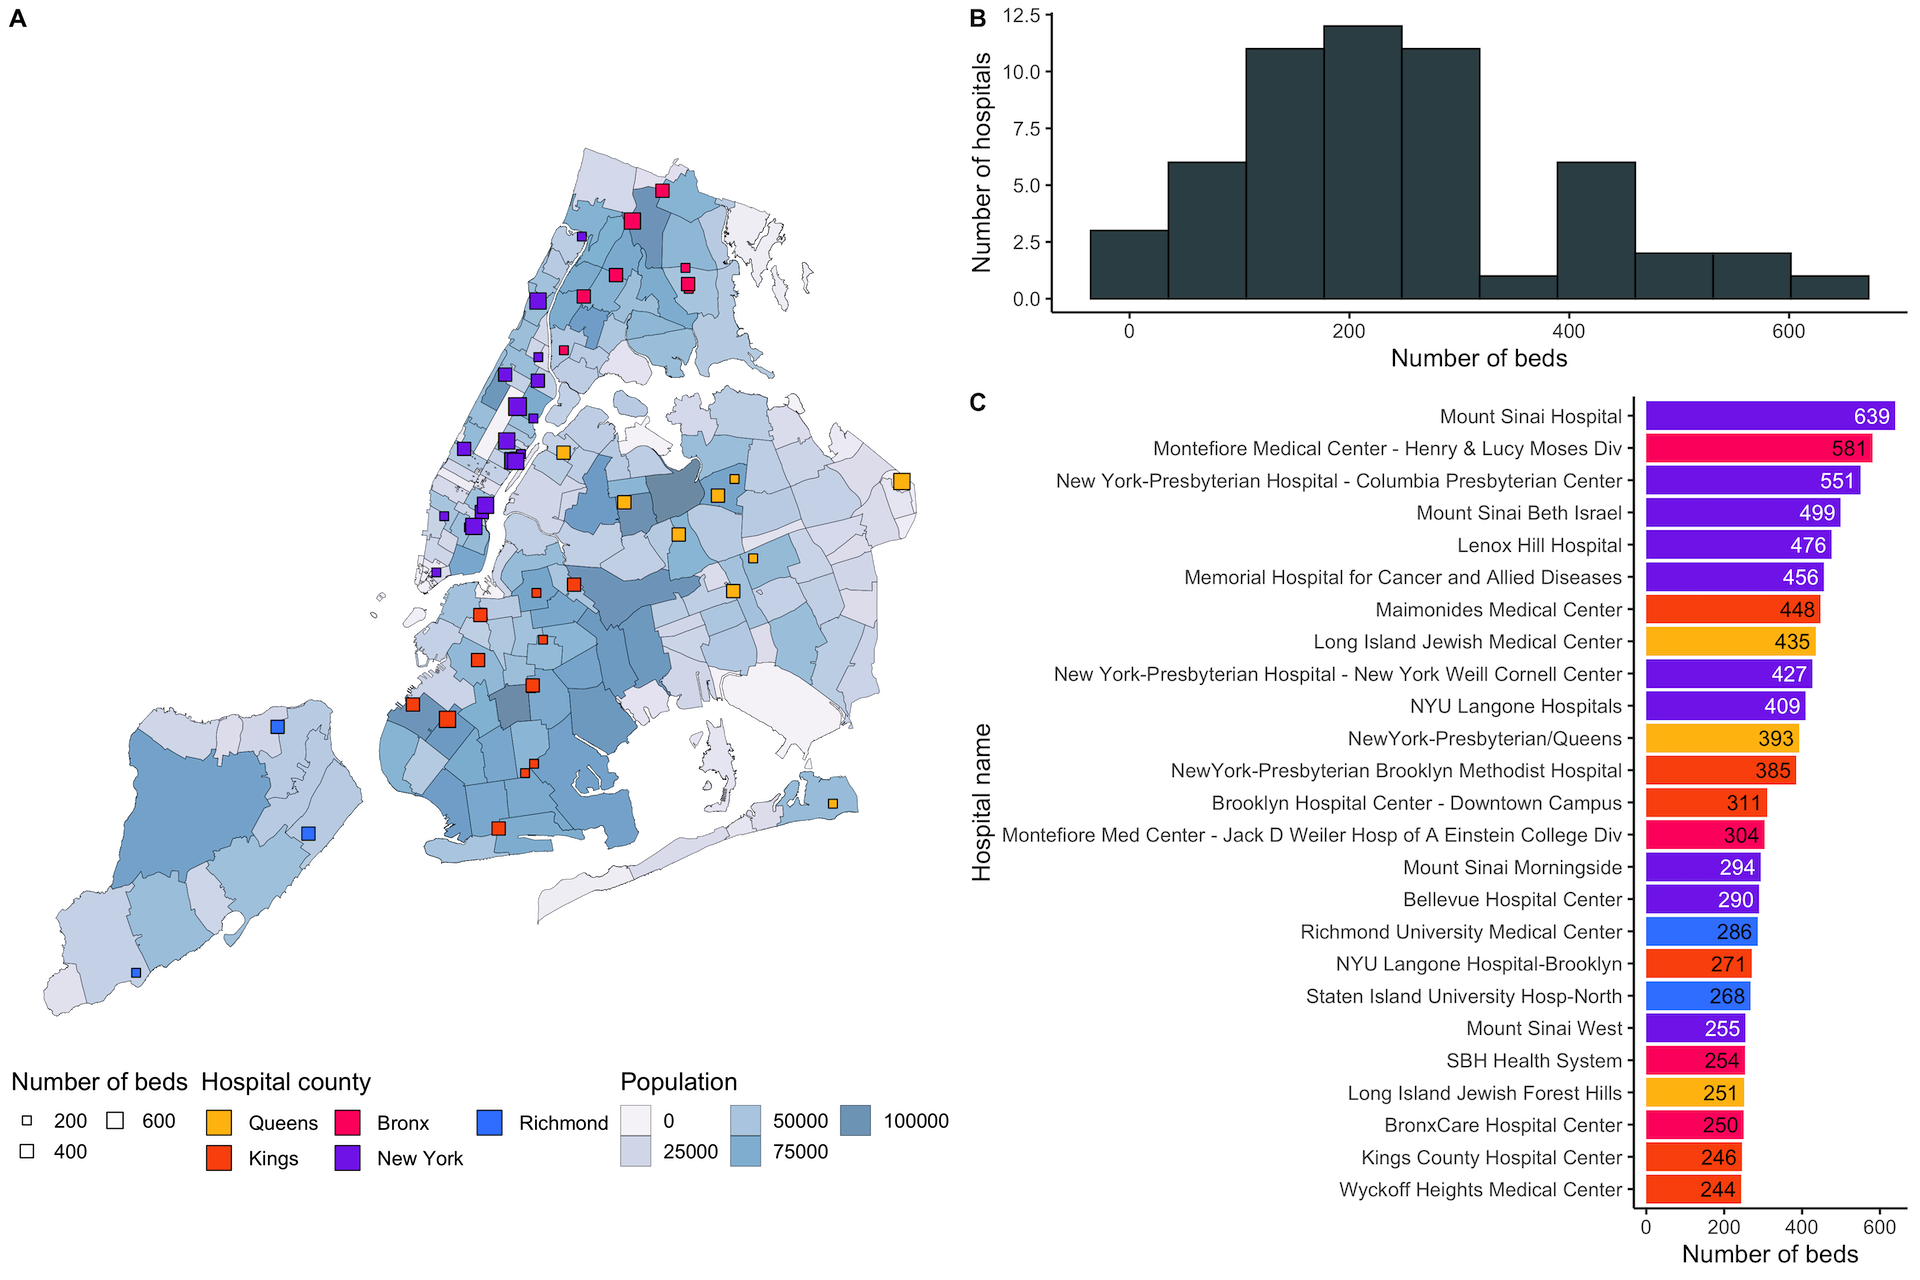
\includegraphics[width=\textwidth]{images/routes/fig1.png}
    \centering
    \caption{
        Patients routes in metropolitan France. GPS routes with more than 5 patients are shown on map (A). Municipalities are colored by the average travel duration for patients with cancer. Patients who visit \ac{clcc} and \ac{chru} hospitals have longer travel durations (B); as well as patients who live in non-dense municipalities (C).
    }
    \label{fig:routes-duration-france}
\end{figure}

\begin{figure}[h]
    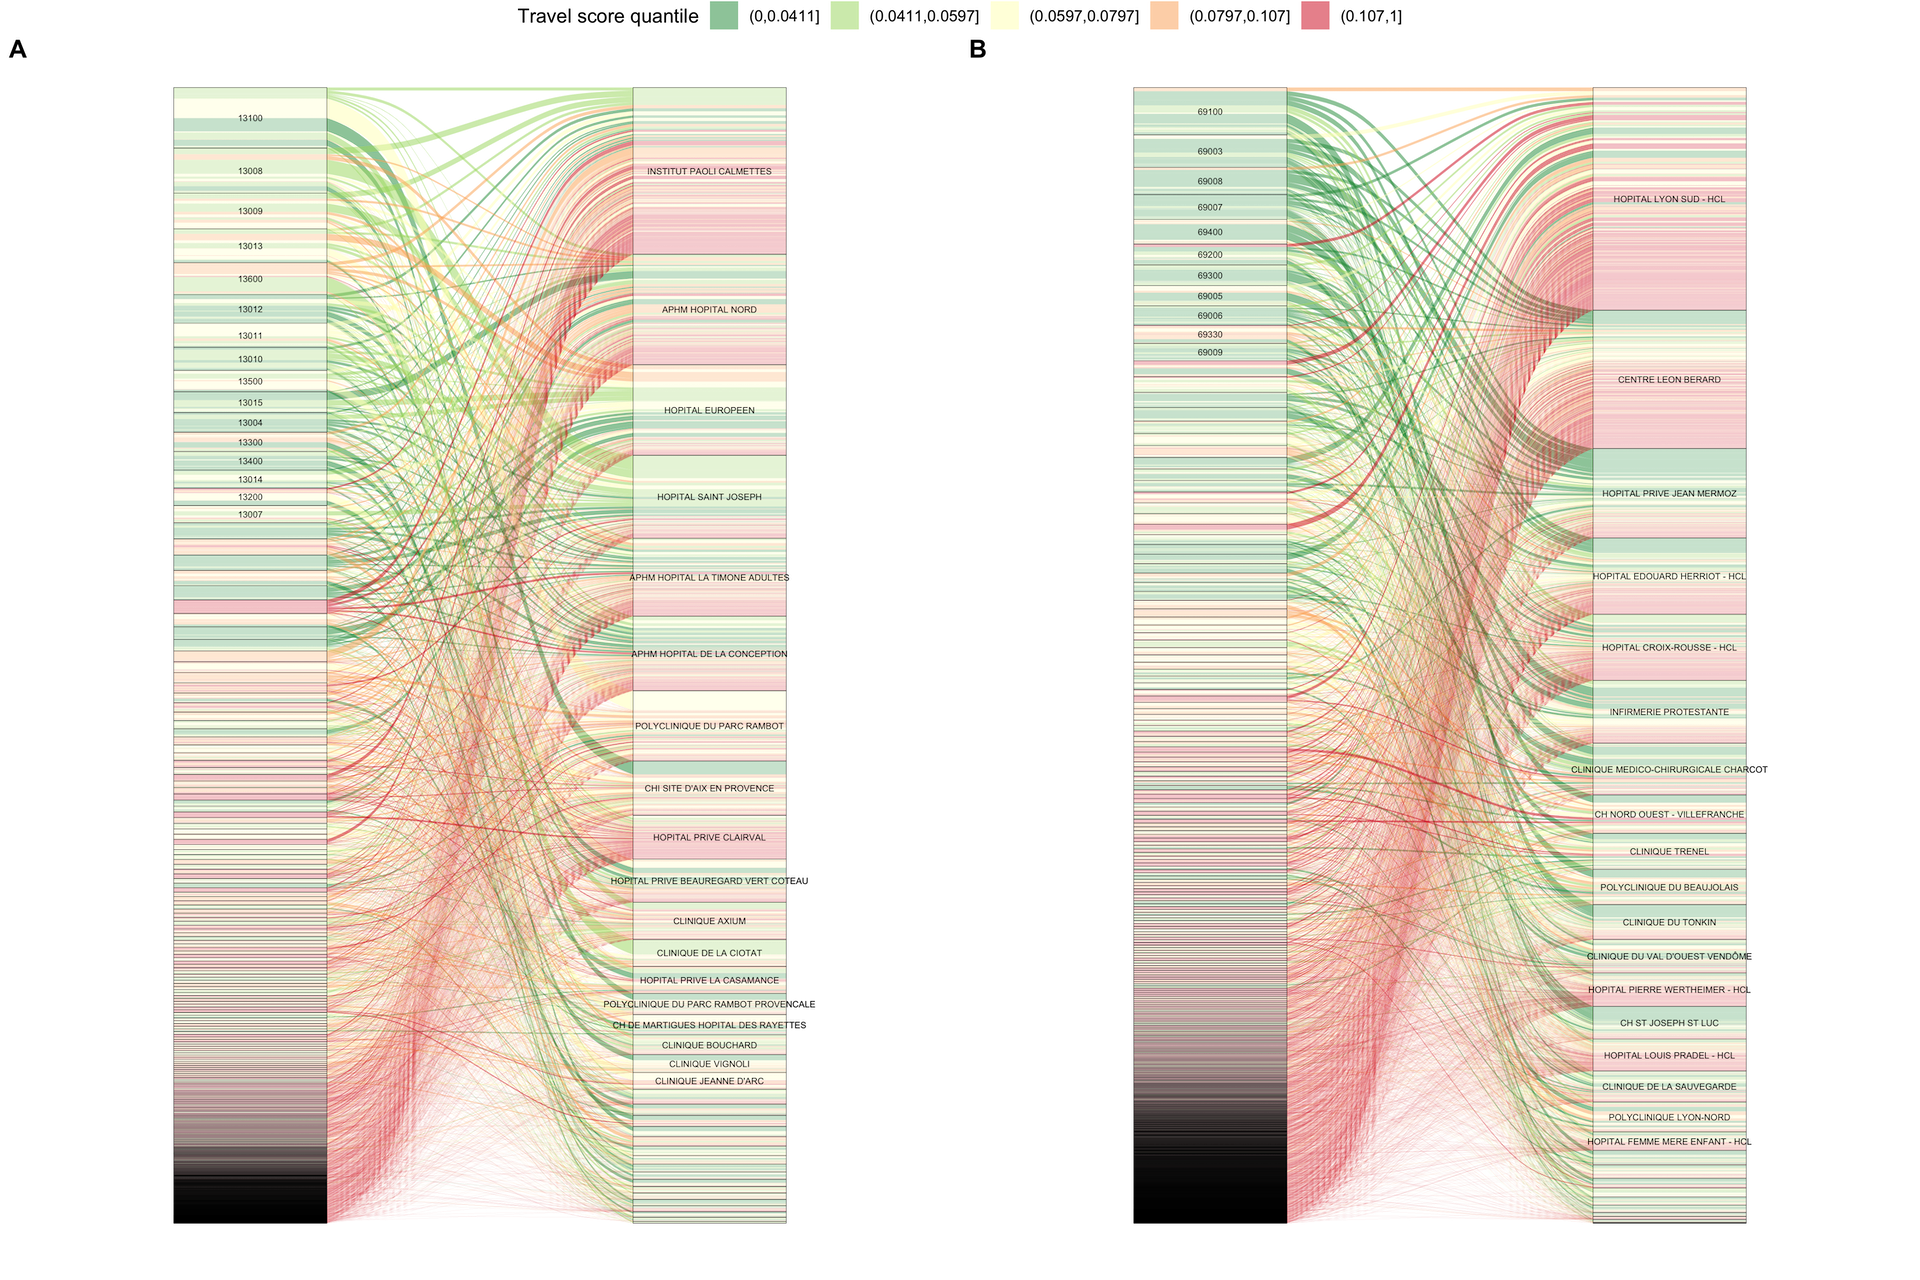
\includegraphics[width=\textwidth]{images/routes/fig6.png}
    \centering
    \caption{
        Distribution of patients traveling to care centers located in Bouches-du-Rhone department. Municipalities are displayed on the right side of the alluvial plot, and care centers on the left side. Municipalities are sized by the number of residing patients. Care centers are sized by the number of treated patients. Flows represent patients travel and are sized by the number of patients traveling from a municipality to a care center. The flows are colored based on the travel score quantile. We can easily identify that the patients living in smaller municipalities are more likely to experience tedious travel. Larger care centers often receive patients from these smaller municipalities.
    }
    \label{fig:routes-alluvial-13}
\end{figure}

\begin{figure}[h]
    \includegraphics[width=\textwidth]{images/routes/fig8.png}
    \centering
    \caption{
        Patients travel, sized by number of travels, and colored by \ac{co2} emission. We study the patients travel in Bourg-en-Bresse area, a sub-urban and rural area located in Auvergne-Rhone-Alpes region. Plot (A) displays the patients flows from municipalities on the right to care centers on the left, similarly to Figure 5. The flows are colored by the resulting \ac{co2} emissions. \ac{co2} emissions are calculated by multiplying the travel distance by the number of travels and the car average consumption. We can see that the higher \ac{co2} emissions are not issued by travels with lots of patients, but instead from travels with fewer patients but much longer drives. This is emphasized on plot (B), showing the \ac{co2} emissions resulting from patients living in Bourg en Bresse area. Indeed, the 42 travels to Hopital Lyon Sud emitted three times as much \ac{co2} than the 253 travels to Centre Hospitalier de Fleyriat.
    }
    \label{fig:routes-co2-01}
\end{figure}
